\documentclass[11pt, oneside]{article}   	% use "amsart" instead of "article" for AMSLaTeX format
\usepackage{geometry}                		% See geometry.pdf to learn the layout options. There are lots.
\geometry{letterpaper}                   		% ... or a4paper or a5paper or ... 
%\geometry{landscape}                		% Activate for for rotated page geometry
%\usepackage[parfill]{parskip}    		% Activate to begin paragraphs with an empty line rather than an indent
\usepackage{graphicx}				% Use pdf, png, jpg, or eps§ with pdflatex; use eps in DVI mode
								% TeX will automatically convert eps --> pdf in pdflatex		
\usepackage{amssymb}
\usepackage{amsmath}
\usepackage{parskip}
\usepackage{color}
\usepackage{hyperref}

\title{Binomial theorem:  proof by induction}
%\author{The Author}
%\section{}
%\subsection*{}
\date{}							% Activate to display a given date or no date

\graphicspath{{/Users/telliott_admin/Dropbox/Tex/png/}}
% \begin{center} 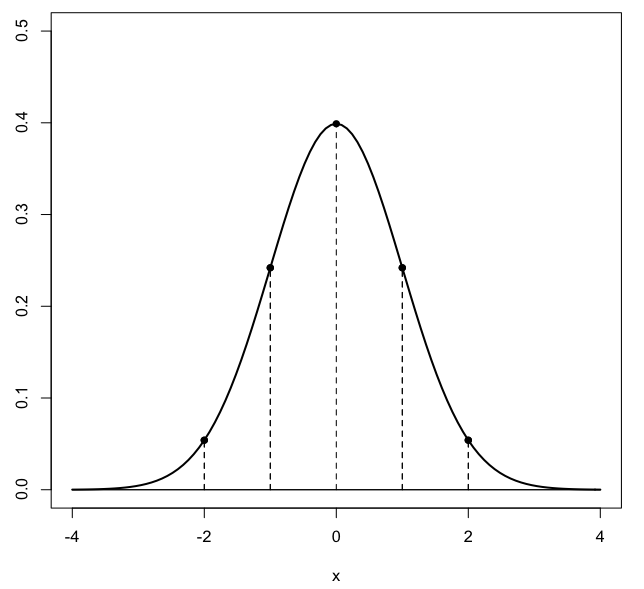
\includegraphics [scale=0.4] {gauss3.png} \end{center}
\begin{document}
\maketitle
\Large
The binomial theorem gives the terms and coefficients of $(a+b)^n$ as follows.  The terms are
\[ (a+b)^n = \sum_{k=0}^{n} c_k \ a^{n-k} \ b^k \]
\[ = c_0 \ a^n + c_1 \ a^{n-1}b + \dots c_{n-1} \ a^2 b^{n-1} + c_n \ b^n \]
where the coefficients are determined by the formula $n$ "choose" $k$ which you may have learned when studying probability.  It is often written as
\[ {n \choose k} = \frac{n!}{k! \ (n-k)!} \]
but can be typeset more simply as $C(n,k)$, so we can rewrite the equation as
\[ (a+b)^n = C(n,0) \ a^n + C(n,1) \ a^{n-1}b + \dots + C(n,n) \ b^n \]
or in summation form as
\[ (a+b)^n = \sum_{k=0}^n C(n,k) \ a^{n-k} b^k \]
(Note that $0!$ is defined to be equal to $1$, partly so that this formula works for the first term)

$C(n,k)$ gives the terms of Pascal's Triangle:
\begin{center} 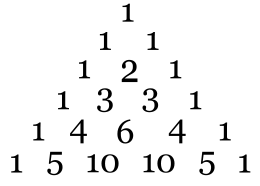
\includegraphics [scale=0.6] {pascal.png} \end{center}
and so on.  

We easily check that this theorem gives the correct values in the expansion of $(a+b)^n$, for small $n$.  For example
\[ (a+b)^2 = (a+b)(a+b) = a^2 + 2ab + b^2 \]
\[ (a+b)^3 = (a+b)(a^2 + 2ab + b^2) = a^3 + 3a^2b + 3ab^2 + b^3 \]
\[ (a+b)^4 = (a+b)(a^3 + 3a^2b + 3ab^2 + b^3) \]
\[ = a^4 + 4a^3b + 6a^2b^2 +  4ab^3 + b^4 \]

As an example of computing any particular coefficient, the second-to-last line is $n=4$ and $k = 0 \rightarrow n$, so the third term ($k=2$) is 
\[ C(4,2) = \frac{4!}{2!(4-2)!} = \frac{4 \cdot 3 \cdot 2}{2 \cdot 2} = 6\]
while for $n=5$ and $k=2$ we have:
\[ C(5,2) = \frac{5!}{2!(5-2)!} = \frac{5 \cdot 4 \cdot 3 \cdot 2}{2 \cdot 3 \cdot 2} = 10 \]

\subsection*{simplification}
You may have noticed that in the above calculations, there are terms that cancel.  We expand $n!$ partially
\[ n! = n \cdot (n-1) \dots (n-k+1) \cdot (n-k)! \]
The last term is also present in the denominator of our formula
\[ C(n,k) = \frac{n!}{k! \ (n-k)!} \]
so we can simplify 
\[ C(n,k) = \frac{n \cdot (n-1) \dots (n-k+1)}{k!} \]

We will be interested in coefficients with $k+1$, so let's take a look at $n$ "choose" $k+1$.  The original definition would give:
\[ C(n,k+1) = \frac{n!}{(k+1)! \ (n-(k+1))!}  \]
Remove one set of parentheses
\[ = \frac{n!}{(k+1)! \ (n-k-1)!}  \]
By the same argument, expand $n!$
\[ = \frac{n \cdot (n-1) \dots (n-k+1) \cdot (n-k) \cdot (n-k-1)!}{(k+1)! \ (n-k-1)!}  \]
\[ = \frac{n \cdot (n-1) \dots (n-k+1) \cdot (n-k)}{(k+1)!} \]
You should convince yourself that the last term in the numerator is correct.  It is somewhat counterintuitive that for $k+1$ the last term is $(n-k)$ (rather than say, $(n-k+2)$, as I thought at first).
\subsection*{induction}
Now we wish to use induction to show that if the formula works for $n$, it also works for $n+1$.
\[ (a+b)^{n} = c_0 \ a^n + c_1 \ a^{n-1}b + \dots c_{n-1} \ a b^{n-1} + c_n \ b^n  \]
\[ (a+b)^{n+1} =  (a+b) \ [ c_0 \ a^n + c_1 \ a^{n-1}b + \dots c_{n-1} \ a b^{n-1} + c_n \ b^n \ ] \]
When we do the multiplication we will have terms on the "ends" containing only powers of $a^{n+1}$ or $b^{n+1}$, and these will retain the same coefficients, namely
\[ c_0 = c_n = 1 \]

For the rest of the terms each one will have two contributions, one from multiplying one term from previous line by $b$, and one from multiplying the next term by $a$.

Let's start by considering a concrete example:  the second ($k=1$) and third ($k=2$) terms in the expansion for $(a+b)^n$:
\[ C(n,1) \ a^{n-1} b + C(n,2) \ a^{n-2}b^2 \]
We multiply the first term by $b$ and the second by $a$, obtaining
\[ C(n,1) \ a^{n-1} b^2 + C(n,2) \ a^{n-1}b^2 \]
\[ = \ [ \ C(n,1)  + C(n,2) \ ] \ a^{n-1}b^2 \]

It isn't so easy to see from looking at the power of $a$ because we are still numbering according to the initial expansion for $(a+b)^n$, but clearly this is the third term in the expansion for $(a+b)^{n+1}$ because it contains $b^2$.

The coefficient for this term according to the binomial theorem or formula should be $C(n+1,2)$.  So, for the proof by induction, we must show that
\[ C(n,1)  + C(n,2) = C(n+1, 2) \]
Generalizing from this, we need
\[ C(n,k) + C(n,k+1) = C(n+1,k+1) \]
That is what we will prove.
\subsection*{coefficient}
Let us examine the general statement
\[ C(n,k) + C(n,k+1) \]
Rewriting it as the factorial using the simplification we found above
\[ \frac{n \cdot (n-1) \dots (n-k+1)}{k!} + \frac{n \cdot (n-1) \dots (n-k+1) \cdot (n-k)}{(k+1)!} \]
We can factor out $(n-k)/(k+1)$ from the second term:
\[ = (\frac{n-k}{k+1}) \ \cdot \frac{n \cdot (n-1) \dots \ (n-k+1) }{k!}  \]
and now this is just that factor multiplied by the first term.

So the complete sum becomes
\[ \ [ \ 1 + (\frac{n-k}{k+1})  \ ] \  \cdot \frac{n \cdot (n-1) \dots \ (n-k+1) }{k!}  \]
Take the leading factor and put it over a common denominator
\[ \frac{(k+1) + (n-k)}{k+1} = \frac{n+1}{k+1} \]
so the sum now becomes
\[ = ( \frac{n+1}{k+1} ) \  \cdot \frac{n \cdot (n-1) \dots \ (n-k+1) }{k!}  \]
\[ = \frac{(n+1) \cdot n \cdot (n-1) \dots \ (n-k+1) }{(k+1)!}  \]
rearranging the last term in the numerator slightly
\[ = \frac{(n+1) \cdot n \cdot (n-1) \dots \ ((n+1)-k) }{(k+1)!}  \]
\[ = C(n+1,k+1) \]
This is the correct expression for $n+1$ (because it has $n+1$ in the right places), and it is the correct expression for $k+1$ because it ends with $n+1$ minus $k$ (rather than $k+1$).  Go back to the simplification section to see this.
\subsection*{recap}
We assume that $C(n,k)$ is the correct coefficient for $a^{n-k}b^k$ in the expansion of $(a+b)^n$, and that $C(n,k+1)$ is the correct coefficient for the succeeding term $a^{n-(k+1)}b^{k+1}$ in the same expansion.  Multiplication of the first by $b$ and the second by $a$ leads to:
\[ \ [ \ C(n,k) + C(n,k+1) \ ] \ a^{n-k}b^{k+1} \]
We need to tweak one exponent slightly when considering this as part of the  expansion for $(a+b)^{n+1}$.  The $n$ in the exponent for $a$ should be expressed in terms of $n$ referring to the incremented value $n+1$ so it needs to step down one unit, becoming $a^{n-k - 1}$ which is equal to $a^{n-(k+1)}$ .  Thus we have
\[ \ [ \ C(n,k) + C(n,k+1) \ ] \ a^{n-(k+1)}b^{k+1} \]
We showed that 
\[ C(n,k) + C(n,k+1) = (1 + \frac{n-k}{k+1}) \cdot  C(n,k) \]
\[ = \frac{n+1}{k+1}) \cdot  C(n,k) \]
\[ = C(n+1,k+1) \]
which is what the binomial theorem gives.  This completes the proof by induction.
$\square$

It is worth looking back at Pascal's Triangle
\begin{center} 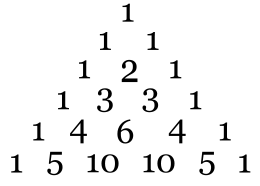
\includegraphics [scale=0.6] {pascal.png} \end{center}
 and recognizing that all we have really done is to show that, indeed, when we take two successive terms in the $k$ and $k+1$ positions, multiplying the first by $b$ and the second by $a$, we generate the coefficient of the $k+1$ term in the row below by adding the first two coefficients.

\end{document}  